\documentclass[document.tex]{subfiles} 
\begin{document}

\clearpage

\subsection{Цифровые компараторы}
Цифровой компаратор или компаратор амплитуд является электронным устройством,
берущим два числа в двоичном виде и определяющим, является ли первое число
меньшим, большим или равным второму числу. Чтобы определить наибольшее из двух
двоичных чисел, рассматриваются отношение величин пар значащих цифр, начиная с
наиболее значащих битов, последовательно продвигаясь к младшим значащим битам до
нахождения неравенства~\cite{wikicmp}.

Вся кодовая база цифровых компараторов находится в пакете devices.cmp и
наследуется от абстрактного класса Device.

\subsubsection{Логическая эквиваленция}

Устройство поразрядной эквиваленции описывается следующим образом:
\begin{equation}
\label{eq:eq}
\forall x: E_x = \overline{F_x \oplus S_x} 
\end{equation}

В выражении~\ref{eq:eq}:
\begin{itemize}[noitemsep]
  \item $x$ -- индекс входного разряда первого и второго операнда;
  \item $F$ -- набор входных разрядов первого операнда;
  \item $S$ -- набор входных разрядов второго операнда;
  \item $E$ -- набор выходных разрядов.
\end{itemize}

\clearpage

Описание поразрядной эквиваленции в разрабатываемой библиотеке представлено в
листинге~\ref{lst:eq}.

\begin{listing}[ht]
\begin{minted}[linenos=true]{python}
class DeviceEq(Device):
    """Equality device"""
    mandatory_signals = ('strobe_signals', 'first_signals', 
                         'second_signals', 'output_signals',)
    mandatory_signals_using_subs = ('strobe_signals',)
    truth_table_signals = ('strobe_signals', 'first_signals', 
                           'second_signals', 'output_signals',)
    constraints = {
        'strobe_signals': {
            'min': 1,
            'max': 10
        },
        'first_signals': {
            'min': 1,
            'max': 7
        },
        'second_signals': {
            'min': 1,
            'max': 7
        },
        'output_signals': {
            'min': 1,
            'max': 7
        }
    }
\end{minted}
\caption{Программное описание класса эквиваленции}
\label{lst:eq}
\end{listing}

\clearpage
В листинге~\ref{lst:eqgen} представлен код для программного синтеза
устройства эквиваленции с 2 входными разрядами первого операнда
(first\_signals='f:2'), 2 входными разрядами второго операнда
(second\_signals='s:2'), 1 прямым входным разрядом строб-сигнала
(strobe\_signals='z:1') и 2 выходными разрядами (output\_signals='o:2').

\begin{listing}[ht]
\begin{minted}{pycon}
>>> from circuitry.devices.cmp import DeviceEq           
>>> pprint(                                                
...     DeviceEq(strobe_signals='z:1', first_signals='f:2',
...              second_signals='s:2', output_signals='o:2',
...              strobe_signals_subs=dict(z0=1))
... )
{'first_signals': (f0, f1),
 'functions': [And(Or(Not(f0), s0), Or(Not(s0), f0), z0),
               And(Or(Not(f1), s1), Or(Not(s1), f1), z0)],
 'output_signals': (o0, o1),
 'second_signals': (s0, s1),
 'strobe_signals': (z0,),
 'strobe_signals_function': z0,
 'strobe_signals_subs': {'z0': 1},
 'strobe_signals_truth_table': [1],
 'truth_table': [([1], [0, 0], [0, 0], [1, 1]),
                 ([1], [0, 0], [1, 0], [0, 1]),
                 ([1], [0, 0], [0, 1], [1, 0]),
                 ([1], [0, 0], [1, 1], [0, 0]),
                 ([1], [1, 0], [0, 0], [0, 1]),
                 ([1], [1, 0], [1, 0], [1, 1]),
                 ([1], [1, 0], [0, 1], [0, 0]),
                 ([1], [1, 0], [1, 1], [1, 0]),
                 ([1], [0, 1], [0, 0], [1, 0]),
                 ([1], [0, 1], [1, 0], [0, 0]),
                 ([1], [0, 1], [0, 1], [1, 1]),
                 ([1], [0, 1], [1, 1], [0, 1]),
                 ([1], [1, 1], [0, 0], [0, 0]),
                 ([1], [1, 1], [1, 0], [1, 0]),
                 ([1], [1, 1], [0, 1], [0, 1]),
                 ([1], [1, 1], [1, 1], [1, 1])]}
\end{minted}
\caption{Программный синтез устройства эквиваленции}
\label{lst:eqgen}
\end{listing}

\clearpage

На рисунке~\ref{fig:deviceeq} представлено условно-графическое обозначение
синтезированного устройства эквиваленции.

\begin{figure}[here]
\centering
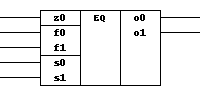
\includegraphics{devices_eq_sym}
\caption{Условно-графическое обозначение устройства эквиваленции}
\label{fig:deviceeq}
\end{figure}

На рисунке~\ref{fig:deviceeqmat} представлено устройство
синтезированной эквиваленции в виде модели Simulink.

\begin{figure}[here]
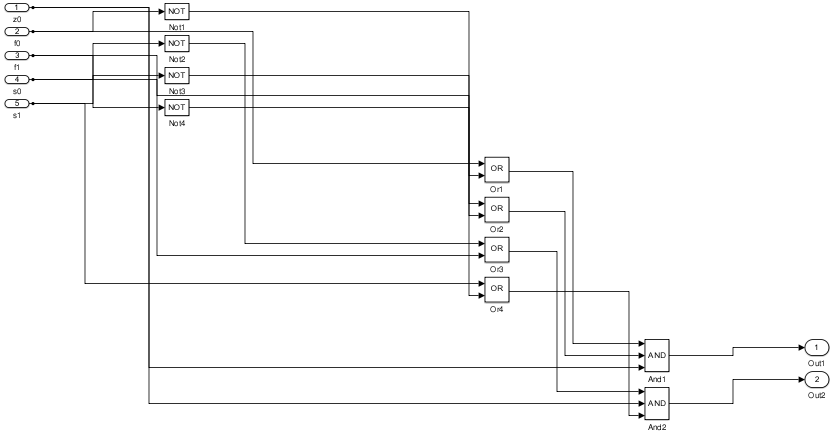
\includegraphics[width=1\linewidth]{devices_eq_mat}
\caption{Представление эквиваленции в виде модели Simulink}
\label{fig:deviceeqmat}
\end{figure}

\clearpage
\subsubsection{Цифровой компаратор}
Устройство цифрового компаратора использует в качестве базового устройство
эквиваленции и описывается следующим образом, используя выражение~\ref{eq:eq}:

\begin{equation}
\label{eq:cmpl}
L_0 = (\overline{F_0} \wedge S_0 \wedge E_1) \vee (\overline{F_1} \wedge
S_1 \wedge E_2) \vee \ldots \vee (\overline{F_n} \wedge S_n)
\end{equation}

\begin{equation}
\label{eq:cmpe}
Q_0 = E_0 \wedge E_1 \wedge \ldots \wedge E_n
\end{equation}

\begin{equation}
\label{eq:cmpg}
G_0 = (F_0 \wedge \overline{S_0} \wedge E_1) \vee (F_1 \wedge \overline{S_1}
\wedge E_2) \vee \ldots \vee (F_n \wedge \overline{S_n})
\end{equation}

\begin{equation}
\label{eq:cmpo}
O = (L_0, Q_0, G_0)
\end{equation}

В выражениях~\ref{eq:cmpl},~\ref{eq:cmpe},~\ref{eq:cmpg}~и~\ref{eq:cmpo}:
\begin{itemize}[noitemsep]
  \item $n$ -- количество входных разрядов первого и второго операнда;
  \item $F$ -- набор входных разрядов первого операнда;
  \item $S$ -- набор входных разрядов второго операнда;
  \item $L_0$ -- разряд, показывающий, что первый операнд меньше второго;
  \item $Q_0$ -- разряд, показывающий, что первый операнд равен второму;
  \item $G_0$ -- разряд, показывающий, что первый операнд больше второго;
  \item $O$ -- набор выходных разрядов.
\end{itemize}

Описание цифрового компаратора в разрабатываемой библиотеке представлено в
листинге~\ref{lst:cmp}.

\begin{listing}[ht]
\begin{minted}[linenos=true]{python}
class DeviceCmp(DeviceEq):
    """Digital comparator device"""
\end{minted}
\caption{Программное описание класса цифрового компаратора}
\label{lst:cmp}
\end{listing}

\clearpage
В листинге~\ref{lst:cmpgen} представлен код для программного синтеза
цифрового компаратора с 2 входными разрядами первого операнда
(first\_signals='f:2'), 2 входными разрядами второго операнда
(second\_signals='s:2'), 1 прямым входным разрядом строб-сигнала
(strobe\_signals='z:1') и 3 выходными разрядами (output\_signals='o:3').

\begin{listing}[ht]
\begin{minted}{pycon}
>>> pprint(                                                                                             
...     DeviceCmp(strobe_signals='z:1', first_signals='f:2',                                            
...               second_signals='s:2', output_signals='o:3',                                           
...               strobe_signals_subs=dict(z0=1))                                                        
... )
{'first_signals': (f0, f1),
 'functions': [And(Or(And(Not(f0), Or(Not(f1), s1), 
                          Or(Not(s1), f1), s0, z0), 
                      And(Not(f1), s1)), z0),
               And(Or(Not(f0), s0), Or(Not(f1), s1), 
                   Or(Not(s0), f0), Or(Not(s1), f1), z0),
               And(Or(And(Not(s0), Or(Not(f1), s1), 
                          Or(Not(s1), f1), f0, z0), 
                      And(Not(s1), f1)), z0)],
 'output_signals': (o0, o1, o2),
 'second_signals': (s0, s1),
 'strobe_signals': (z0,),
 'strobe_signals_function': z0,
 'strobe_signals_subs': {'z0': 1},
 'strobe_signals_truth_table': [1],
 'truth_table': [([1], [0, 0], [0, 0], [0, 1, 0]),
                 ([1], [0, 0], [1, 0], [1, 0, 0]),
                 ([1], [0, 0], [0, 1], [1, 0, 0]),
                 ([1], [0, 0], [1, 1], [1, 0, 0]),
                 ([1], [1, 0], [0, 0], [0, 0, 1]),
                 ([1], [1, 0], [1, 0], [0, 1, 0]),
                 ([1], [1, 0], [0, 1], [1, 0, 0]),
                 ([1], [1, 0], [1, 1], [1, 0, 0]),
                 ([1], [0, 1], [0, 0], [0, 0, 1]),
                 ([1], [0, 1], [1, 0], [0, 0, 1]),
                 ([1], [0, 1], [0, 1], [0, 1, 0]),
                 ([1], [0, 1], [1, 1], [1, 0, 0]),
                 ([1], [1, 1], [0, 0], [0, 0, 1]),
                 ([1], [1, 1], [1, 0], [0, 0, 1]),
                 ([1], [1, 1], [0, 1], [0, 0, 1]),
                 ([1], [1, 1], [1, 1], [0, 1, 0])]}
\end{minted}
\caption{Программный синтез цифрового компаратора}
\label{lst:cmpgen}
\end{listing}

\clearpage

На рисунке~\ref{fig:devicecmp} представлено условно-графическое обозначение
синтезированного устройства цифрового компаратора.

\begin{figure}[here]
\centering
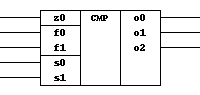
\includegraphics{devices_cmp_sym}
\caption{Условно-графическое обозначение цифрового компаратора}
\label{fig:devicecmp}
\end{figure}

На рисунке~\ref{fig:devicecmpmat} представлено устройство
синтезированного цифрового компаратора в виде модели Simulink.

\begin{figure}[here]
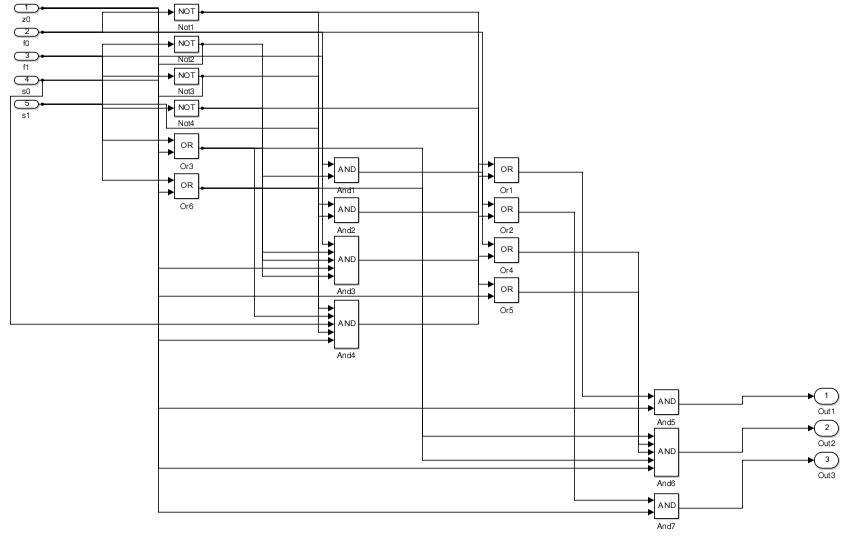
\includegraphics[width=1\linewidth]{devices_cmp_mat}
\caption{Представление цифрового компаратора в виде модели Simulink}
\label{fig:devicecmpmat}
\end{figure}

\end{document}